\documentclass[12pt,letterpaper]{article}
\usepackage{fullpage}
\usepackage[top=2cm, bottom=4.5cm, left=2.5cm, right=2.5cm]{geometry}
\usepackage{amsmath,amsthm,amsfonts,amssymb,amscd}
\usepackage{lastpage}
\usepackage{enumerate}
\usepackage{fancyhdr}
\usepackage{mathrsfs}
\usepackage{xcolor}
\usepackage{graphicx}
\usepackage{listings}
\usepackage{mcode}
\usepackage{hyperref}
\usepackage{movie15}
\usepackage{hyperref}

% \hypersetup{%
%   colorlinks=true,
%   linkcolor=blue,
%   linkbordercolor={0 0 1}
% }
 
% \renewcommand\lstlistingname{Algorithm}
% \renewcommand\lstlistlistingname{Algorithms}
% \def\lstlistingautorefname{Alg.}

% \lstdefinestyle{Python}{
%     language        = Python,
%     frame           = lines, 
%     basicstyle      = \footnotesize,
%     keywordstyle    = \color{blue},
%     stringstyle     = \color{green},
%     commentstyle    = \color{red}\ttfamily
% }

\setlength{\parindent}{0.0in}
\setlength{\parskip}{0.05in}

% Edit these as appropriate
\newcommand\course{Mobile Robotics}
\newcommand\hwnumber{1}                  % <-- homework number
\newcommand\NetIDa{mk05198}           % <-- NetID of person #1
\newcommand\NetIDb{}           % <-- NetID of person #2 (Comment this line out for problem sets)

\pagestyle{fancyplain}
\headheight 35pt
\lhead{\NetIDa}
\lhead{\NetIDa\\\NetIDb}                 % <-- Comment this line out for problem sets (make sure you are person #1)
\chead{\textbf{\Large Homework \hwnumber}}
\rhead{\course \\ \today}
\lfoot{}
\cfoot{}
\rfoot{\small\thepage}
\headsep 1.5em

\begin{document}

\section*{Task 1}



\begin{enumerate}
  \item
   \textbf{Velocities}: \\
   Velocities for the robot are taken as derivative of its trajectory. The following listing shows generation of trajectory and velocity calculations. The velocity vectors are augmented with a zero to match the size of the trajectory vectors.
\begin{lstlisting}
clc;close all 
N = 500; 
t = linspace(-pi, pi, N); 

x = 8*(sin(t)).^3; 
y = 8*(sin(2*t)).^3; 

vx = gradient(x, 2*pi/N);
vy = gradient(y, 2*pi/N);
\end{lstlisting}
  \item
\textbf{Acceleration}:\\
Taking time derivatives of the velocity vectors, we get acceleration as: 

\begin{lstlisting}
ax = gradient(vx, 2*pi/N);
ay = gradient(vy, 2*pi/N);
\end{lstlisting}

\item 
\textbf{Robot Velocities}:\\
Using expression (1) and (3) from the assignment prompt, we calculate velocities as follows: 
\begin{lstlisting}
%orientation
phi = atan2(vy, vx); 

%robot velocities
v = vx.*cos(phi) + vy.*sin(phi); 
omega = (vx.*ay - vy.*ax)./(vx.^2+vy.^2); 

%Plotting
subplot(2, 1, 1)
plot(v, 'linewidth', 4) 
xlabel('time',  'FontSize', 14)
ylabel('velocity',  'FontSize', 14)
title('Linear velocity', 'FontSize', 18)

subplot(2, 1, 2)
plot(omega, 'linewidth', 4)
title('Angular velocity', 'FontSize', 18)
xlabel('time',  'FontSize', 14)
ylabel('velocity',  'FontSize', 14)
print -deps figures/task1 
\end{lstlisting}

Run the above presented code in chronological order, we get the following velocity plots:

\begin{figure} [h]
    \centering
    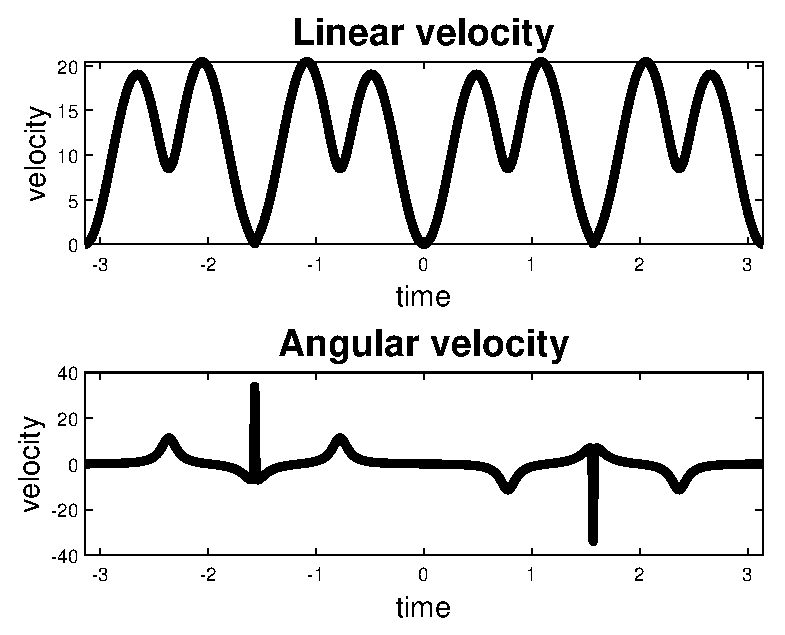
\includegraphics[]{figures/task1_velocities.eps}
    \caption{velocities}
    \label{fig:my_label}
\end{figure}

\item 
\textbf{Trajectory traversal}:\\
The following code creates an animated gif with the point mobile node traversing the given trajectory: 
\begin{lstlisting}
h = figure; 
axis tight manual % this ensures that getframe() returns a consistent size
filename = 'figures/task1_trajectory.gif'; 
plot(x, y, 'b', 'linewidth', 3)
hold on 
for i=1:10:N      
    plot(x(1:i), y(1:i), 'g-', 'linewidth', 6)
    legend('Given Trajectory', "Robot's Path"); 
    drawnow; 
    
    %create GIF
    frame = getframe(h); 
    im = frame2im(frame); 
    [imind,cm] = rgb2ind(im,256); 
    % Write to the GIF File 
    if i == 1
      imwrite(imind,cm,filename,'gif', 'Loopcount',inf); 
    else 
      imwrite(imind,cm,filename,'gif','WriteMode','append'); 
    end 

end
hold off
\end{lstlisting}
\end{enumerate}
The animation can be found here: \href{https://github.com/mehhdiii/Robot-External-Kinematics/blob/main/figures/output.gif}{/mehhdiii/Robot-External-Kinematics/figures}

\section*{Task 2}
Wheel velocities are obtained using the following script: 
\begin{lstlisting}
W = 1/2; r = 1/4; T=0.1; 

%initialize Inverse kinematics velocities
omega = zeros(1, N); v = zeros(1, N); 
vL = zeros(1, N); vR = zeros(1, N); 
omegaL = zeros(1, N); omegaR = zeros(1, N); 


%initialize resulting forward kinematic variables: 
x_f = zeros(1, N); y_f = zeros(1, N); phi_f = zeros(1, N); 

for n = 2:N-1
    %calculating inverse kinematics variables: 
    mu = 1/2*(sin(phi(n))*(y(n+1)-y(n))+cos(phi(n)*(x(n+1)-x(n))))...
        /(cos(phi(n))*(y(n+1)-y(n))-sin(phi(n))*(x(n+1)-x(n))); 
    x_m = (x(n)+x(n+1))/2; 
    y_m = (y(n)+y(n+1))/2; 
    
    x_star = x_m - mu/2 * (y(n+1) - y(n)); 
    y_star = y_m + mu/2 * (x(n+1)-x(n)); 
    
    R_n = sqrt((x(n) - x_star)^2 + (y(n)-y_star)^2); 
    theta_1 = atan2((y(n)-y_star), (x(n)-x_star)); 
    theta_2 = atan2((y(n+1)-y_star), (x(n+1)-x_star)); 
    del_phi = wrapToPi(theta_1 - theta_2); 
    
    %resulting Inv-Kinematics velocities: 
    omega(n) = del_phi/T; 
    v(n) = R_n*abs(omega(n));  
    vL(n) = (R_n-1/2 *W)*omega(n); 
    vR(n) = (R_n+1/2 *W)*omega(n); 
    omegaL(n) = vL(n)/r; 
    omegaR(n) = vR(n)/r; 

end

figure()
subplot 221
plot(t,vL,'linewidth', 2)
xlabel('time',  'FontSize', 10)
ylabel('velocity',  'FontSize', 10)
title('Left Wheel velocity', 'FontSize', 14)
xlim([-pi  pi])

subplot 222
plot(t,vR, 'linewidth', 2)
xlabel('time',  'FontSize', 10)
ylabel('velocity',  'FontSize', 10)
title('Right Wheel velocity', 'FontSize', 14)
xlim([-pi  pi])

subplot 223
plot(t,omegaL, 'linewidth', 2)
xlabel('time',  'FontSize', 10)
ylabel('velocity',  'FontSize', 10)
xlim([-pi  pi])

title('Left Wheel angular velocity', 'FontSize', 14)
subplot 224
plot(t,omegaR, 'linewidth', 2)
xlabel('time',  'FontSize', 10)
ylabel('velocity',  'FontSize', 10)
title('Right Wheel angular velocity', 'FontSize', 14)
xlim([-pi  pi])

print -deps figures/task2
\end{lstlisting}
\begin{figure} [h]
    \centering
    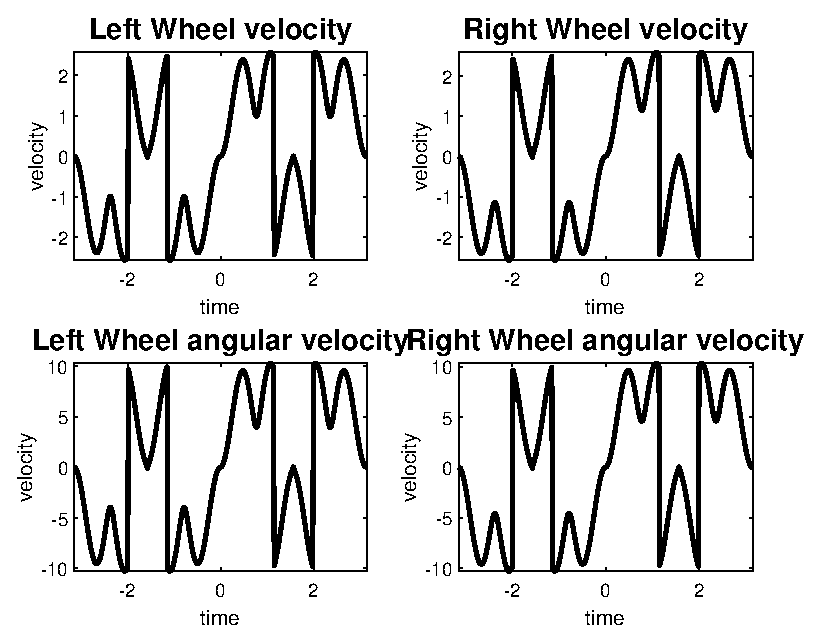
\includegraphics[]{figures/task2.eps}
    \caption{Wheel velocities}
    \label{fig:my_label}
\end{figure}
Complete code can be found at: \href{https://github.com/mehhdiii/Robot-External-Kinematics}{github.com/mehhdiii/Robot-External-Kinematics}
\end{document}
